\documentclass[12pt]{article}

\input preamble

\title{Principles of Parallel Architecture\\
Amdahl’s law and speed up}
\author{Xitong Liu \\
xliu@ece.udel.edu}

\begin{document}

\maketitle

\section{Amdahl�s Law}
\begin{description}
\item[Q:] Assume that your Matrix Multiply program is 0.5\% serial. What is the maximum 
speeding up that you can get using:
	\begin{enumerate}
		\item 2 processors?
		\item 10 processors?
		\item 1000 processors?
		\item 10000 processors?
		\item Infinite Processors?
	\end{enumerate}
	
\item[A:] According to Amdahl�s Law, the speed up 
\begin{equation}
S = \frac{1}{(1-P) + \frac{P}{N}}
\end{equation}
in which $P$ is the parallel part and $N$ is the number of processors. In this case, 
$P = 1 - 0.005 = 0.995$. For different values of $N$, the speed up is:

	\begin{enumerate}
		\item 2 processors, 1.9900
		\item 10 processors, 9.5693
		\item 1000 processors, 169.4915
		\item 10000 processors, 200.0000
		\item Infinite Processors, 200.0000
	\end{enumerate}
	
\end{description}

\end{document}

\begin{comment}
\begin{figure}[h!]
	\begin{center}
		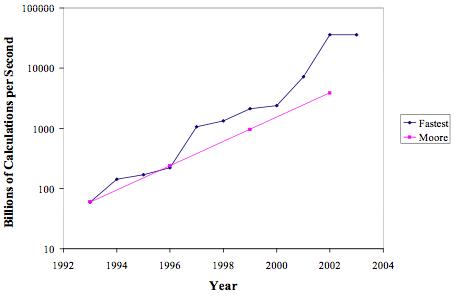
\includegraphics[width=0.7\textwidth, angle=0]{fatest.png}
		\caption{\label{fig:fatest}Fatest SuperComputer in the world}
	\end{center}
\end{figure}
\end{comment}